\chapter{EVENTOS DE EXTENSÃO REALIZADOS}

Infelizmente, não foi possível realizar eventos de extensão durante o período do projeto. No entanto,esperamos poder organizar uma variedade de eventos no futuro, tais como seminários, fóruns, congressos, semanas temáticas, palestras, dinâmicas, oficinas, entre outros, para promover ainda mais o engajamento com a comunidade e disseminar conhecimento sobre programação e robótica.

Porém, durante a execução do projeto, diversas atividades de extensão foram realizadas para promover o aprendizado em computação e compartilhar os resultados obtidos. Dessas atividades, destaca-se a oferta do workshop "Desenvolvimento de Competências para Competições de Robótica com Java". Sendo uma das iniciativas de maior relevância, foi projetado para fornecer aos participantes as habilidades necessárias para se destacarem em competições de robótica utilizando a linguagem de programação Java.

\begin{figure}[H]
    \centering
    \caption{Capa da oferta do workshop "Desenvolvimento de Competências para Competições de Robótica com Java" durante o VI Sercomp.}
    \includegraphics[scale=0.2]{imagens/imagem17.jpg}
\end{figure}

\vspace{2em}

Durante o evento do VI SERCOMP (Congresso Sertanejoo de Computação), os participantes aprenderam os fundamentos da programação em Java e como aplicar esses conhecimentos na programação de robôs para competições de alto nível, como as competições da FTC (First Tech Challenge). Através de uma abordagem prática e focada no desenvolvimento de habilidades específicas, o workshop teve grande impacto.

\begin{figure}[H]
    \centering
    \caption{Participantes do workshop "Desenvolvimento de Competências para Competições de Robótica com Java" em atividade.}
    \includegraphics[scale=0.2]{imagens/imagem16.jpg}
\end{figure}

Além do workshop mencionado, outras atividades de extensão foram realizadas, promovendo o aprendizado em computação e fortalecendo os vínculos entre o projeto e a comunidade acadêmica.

Outro exemplo dessas atividades foi a oferta da Jornada de Atualização em Computação "Introdução à Orientação a Objetos em Java: Conceitos e Exemplos Práticos", realizada durante o VI Semana Zero do Curso de Computação. Neste evento, os participantes tiveram a oportunidade de aprender os princípios fundamentais da programação orientada a objetos, uma base essencial para o desenvolvimento de aplicações em Java.

\begin{figure}[H]
    \centering
    \caption{Oferta da Jornada de Atualização em Computação "Introdução à Orientação a Objetos em Java: Conceitos e Exemplos Práticos" durante o VI Semana Zero do Curso de Computação.}
    \includegraphics[scale=0.18]{imagens/imagem15.jpeg}
\end{figure}

Outro destaque foi o minicurso "Programação em Java: Introdução aos Fundamentos e Sintaxe", oferecido durante o I Congresso de Fluência entre Ensino, Tecnologia e Gestão. Esse minicurso forneceu uma introdução prática à linguagem Java, abordando desde a sintaxe básica até os primeiros conceitos de programação.

\begin{figure}[H]
    \centering
    \caption{Oferta do Minicurso "Programação em Java: Introdução aos fundamentos e sintaxe" durante o I Congresso de Fluência entre Ensino, Tecnologia e Gestão.}
    \includegraphics[scale=0.4]{imagens/imagem14.jpeg}
\end{figure}

Adicionalmente, participamos da Mostra de Extensão durante a VII Semana Zero do Curso de Computação, onde os resultados do projeto foram apresentados. Neste evento, tivemos a oportunidade de compartilhar com a comunidade acadêmica os impactos do "Prognitive", os objetivos atingidos e os planos para as próximas fases do projeto.

\begin{figure}[H]
    \centering
    \caption{Participação na Mostra de Extensão para apresentar os Resultados do Projeto durante a VII Semana Zero do Curso de Computação.}
    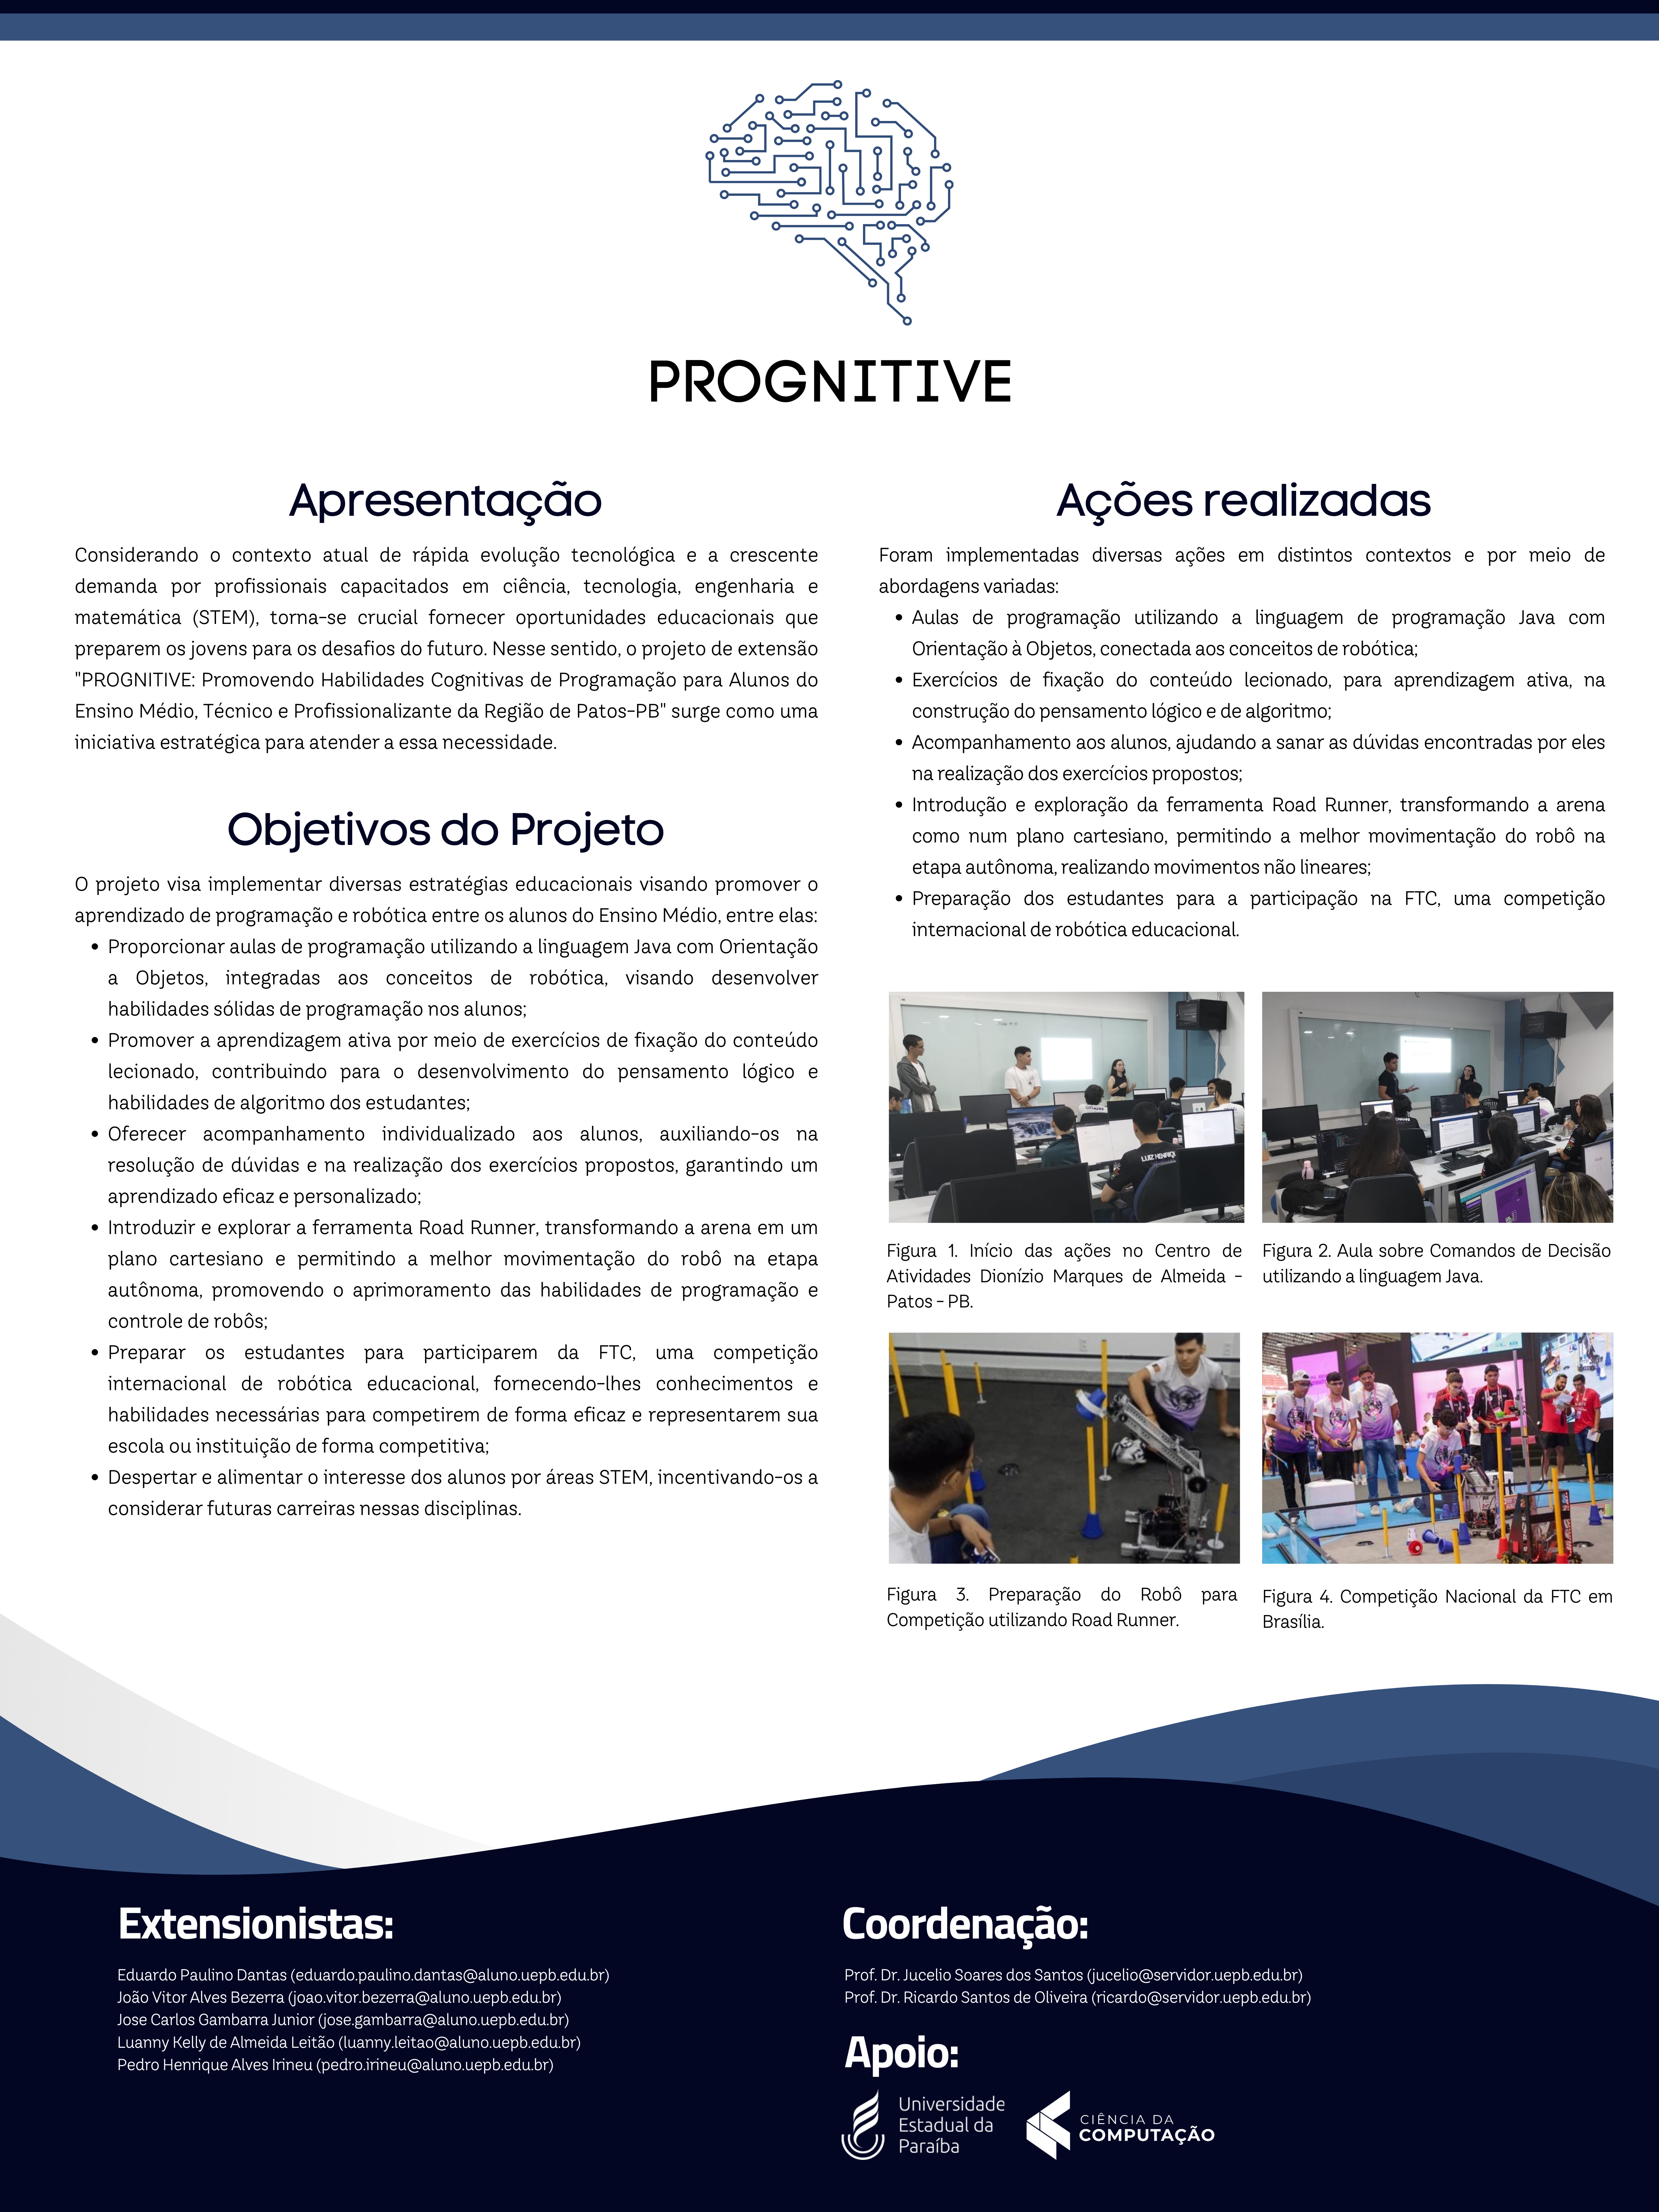
\includegraphics[scale=0.08]{imagens/imagem13.png}
    \includegraphics[scale=0.2125]{imagens/imagem12.jpeg}
\end{figure}

Essas atividades de extensão não apenas contribuíram para a disseminação do conhecimento em computação e robótica, mas também fortaleceram os laços entre a universidade e a comunidade externa. Ao participar de eventos como o VI Semana Zero do Curso de Computação, o I Congresso de Fluência entre Ensino, Tecnologia e Gestão, e a VII Semana Zero do Curso de Computação, conseguimos estabelecer conexões valiosas com estudantes, professores e pesquisadores, ampliando a visibilidade do projeto e atraindo novos colaboradores. Essas iniciativas tiveram um impacto significativo na promoção da educação em ciências exatas e tecnologia, além de proporcionar um ambiente de troca de conhecimentos e experiências.